% Appendix: Routing Latency Microbenchmark

\section{Routing Latency Microbenchmark}
\label{sec:latency_benchmark}

We profile ParetoBandit's per-request routing overhead to validate the
computational-efficiency claims in Section~\ref{sec:efficiency}.
Eight configurations isolate three factors:
\emph{Sherman-Morrison (SM) vs.\ full inversion} (controlled at the same
level of abstraction), \emph{production overhead} (locks, budget pacing,
forgetting), and \emph{PCA dimensionality reduction} ($d{=}26$ vs.\ $d{=}385$).
All configurations use $K{=}3$ arms, synthetic whitened context
vectors, and 4,500 measured route\,+\,update cycles
(500-round warmup excluded).
Context vectors are drawn i.i.d.\ from a standard normal, $\ell_2$-normalised,
and augmented with a bias term---matching the distribution of real
PCA-whitened embeddings in dimensionality and unit-norm structure.
Synthetic vectors are appropriate here because the benchmark targets the
linear-algebra cost of \texttt{route()} and \texttt{update()}, which depends
only on the vector dimension $d$ and the number of arms $K$, not on the
semantic content of the prompt.
Using synthetic inputs eliminates dataset I/O, embedding-model inference, and
PCA projection from the timing loop, ensuring the measurements isolate routing
computation alone.
The full end-to-end pipeline including embedding and PCA is profiled separately
in the E2E breakdown below (Table~\ref{tab:e2e_latency_breakdown}).

\begin{table}[h]
\centering
\caption{Per-request routing latency ($\mu$s) and throughput.
\emph{Bare~SM} is a minimal LinUCB implementation using only the $O(d^2)$
Sherman-Morrison rank-1 update, with no production features.
\emph{Cached~Inv.}\ replaces that update with a full $O(d^3)$
\texttt{np.linalg.inv} call but is otherwise identical---both share the same
\texttt{route()} code path (same Python base class), so any route-latency
difference is measurement noise, cleanly isolating the algorithmic effect.
\emph{ParetoBandit} is the full production router: it uses the SM algorithm
plus locks, budget pacing, forgetting, and staleness tracking.
\emph{Per-Route Inv.}\ is a worst-case strawman that never caches $A^{-1}$,
recomputing it on every \texttt{route()} call.}
\label{tab:latency}
\small
\resizebox{\columnwidth}{!}{%
\begin{tabular}{@{}l r r r r r@{}}
\toprule
 & \multicolumn{2}{c}{\textbf{Route ($\mu$s)}}
 & \multicolumn{2}{c}{\textbf{Update ($\mu$s)}}
 & \textbf{Throughput} \\
\cmidrule(lr){2-3}\cmidrule(lr){4-5}
\textbf{Configuration}
 & p50 & p95 & p50 & p95 & (req/s) \\
\midrule
\multicolumn{6}{@{}l}{\emph{Production (full router with locks, pacing, forgetting)}} \\
ParetoBandit ($d{=}26$)        & \latPBdTwentySixRouteMedian & \latPBdTwentySixRoutePNineFive & \latPBdTwentySixUpdateMedian & \latPBdTwentySixUpdatePNineFive & \latPBdTwentySixThroughput \\
ParetoBandit ($d{=}385$)       & \latPBdFullRouteMedian & \latPBdFullRoutePNineFive & \latPBdFullUpdateMedian & \latPBdFullUpdatePNineFive & \latPBdFullThroughput \\
\addlinespace
\multicolumn{6}{@{}l}{\emph{Algorithmic isolation (identical \texttt{route()}, only \texttt{update()} differs)}} \\
Bare SM ($d{=}26$)             & \latSMdTwentySixRouteMedian & \latSMdTwentySixRoutePNineFive & \latSMdTwentySixUpdateMedian & \latSMdTwentySixUpdatePNineFive & \latSMdTwentySixThroughput \\
Bare SM ($d{=}385$)            & \latSMdFullRouteMedian & \latSMdFullRoutePNineFive & \latSMdFullUpdateMedian & \latSMdFullUpdatePNineFive & \latSMdFullThroughput \\
Cached Inv.\ ($d{=}26$)       & \latCachedDTwentySixRouteMedian & \latCachedDTwentySixRoutePNineFive & \latCachedDTwentySixUpdateMedian & \latCachedDTwentySixUpdatePNineFive & \latCachedDTwentySixThroughput \\
Cached Inv.\ ($d{=}385$)      & \latCachedDFullRouteMedian & \latCachedDFullRoutePNineFive & \latCachedDFullUpdateMedian & \latCachedDFullUpdatePNineFive & \latCachedDFullThroughput \\
\addlinespace
\multicolumn{6}{@{}l}{\emph{Worst-case baseline (never caches $A^{-1}$)}} \\
Per-Route Inv.\ ($d{=}26$)    & \latPerRouteDTwentySixRouteMedian & \latPerRouteDTwentySixRoutePNineFive & \latPerRouteDTwentySixUpdateMedian & \latPerRouteDTwentySixUpdatePNineFive & \latPerRouteDTwentySixThroughput \\
Per-Route Inv.\ ($d{=}385$)   & \latPerRouteDFullRouteMedian & \latPerRouteDFullRoutePNineFive & \latPerRouteDFullUpdateMedian & \latPerRouteDFullUpdatePNineFive & \latPerRouteDFullThroughput \\
\bottomrule
\end{tabular}
}
\end{table}

\begin{figure*}[t]
\centering
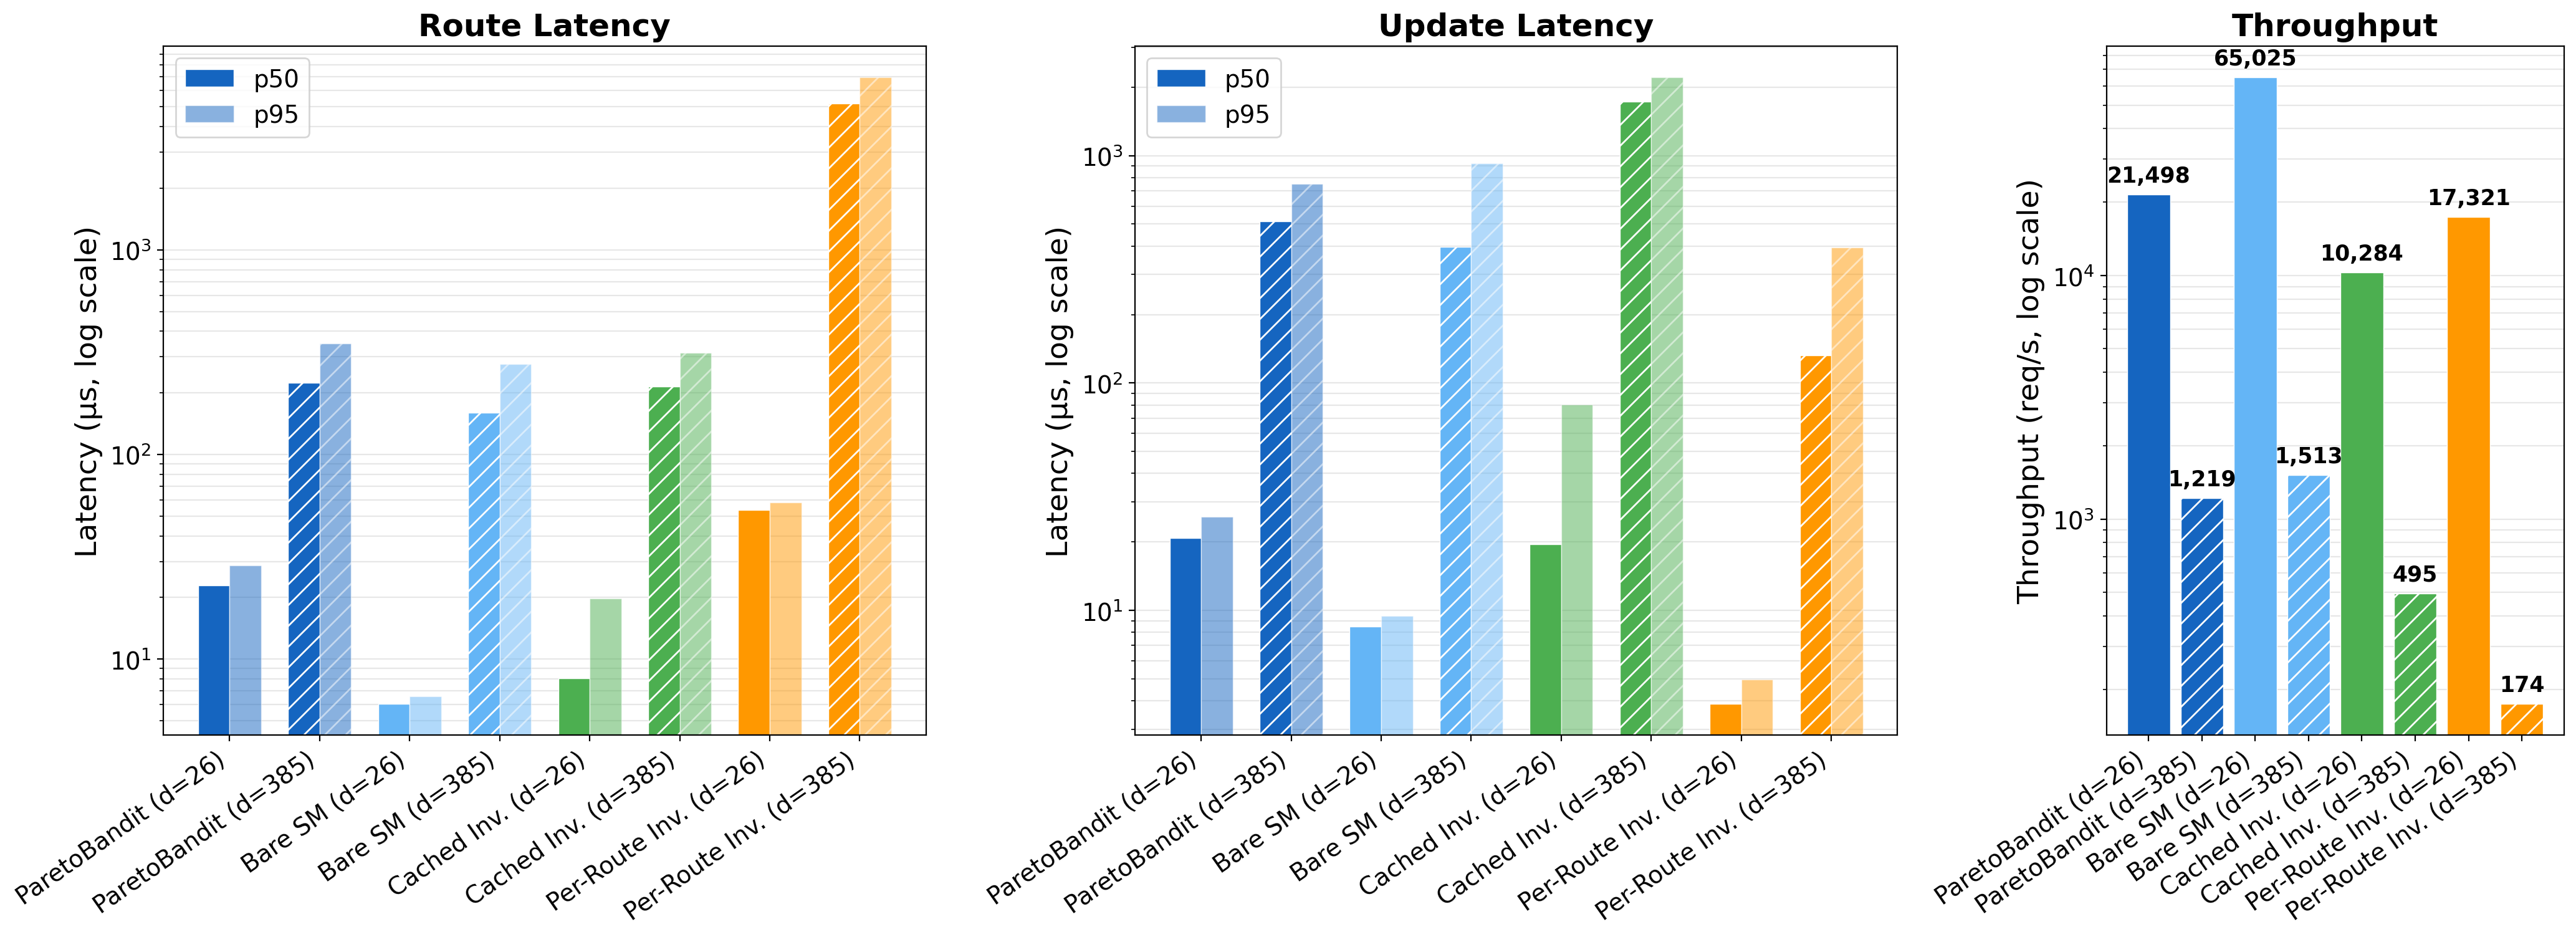
\includegraphics[width=\textwidth]{../experiments/appendix/latency_benchmark/results/latency_benchmark.png}
\caption{Route latency (left), update latency (centre), and throughput
(right) for eight router configurations on a log scale.
Bare~SM and Cached~Inv.\ share identical \texttt{route()} code, so the
route panel confirms they are equivalent; the update panel exposes
Sherman-Morrison's actual contribution ($O(d^2)$ vs.\ $O(d^3)$).
ParetoBandit bars quantify the additional cost of production features.}
\label{fig:latency_benchmark}
\end{figure*}

\paragraph{Algorithmic isolation: SM vs.\ full inversion.}
Bare~SM is a stripped-down LinUCB that applies only the $O(d^2)$
Sherman-Morrison rank-1 update, with no production features (no locks,
pacing, or forgetting).
Cached~Inv.\ is identical except that its \texttt{update()} calls
$O(d^3)$ \texttt{np.linalg.inv} instead of the SM correction.
Both configurations inherit from the same Python base class and execute
\emph{literally the same} \texttt{route()} method (UCB scoring via
cached $A_a^{-1}$ and $\hat\theta_a$), so any route-latency difference
is measurement noise, not code divergence.

\begin{itemize}[nosep,leftmargin=*]
  \item \textbf{Route latency is identical} between Bare~SM and
    Cached~Inv.\ at each dimension (same code path).
  \item \textbf{Update latency} is where SM helps: at $d{=}385$
    the $O(d^2)$ SM update is substantially faster than the $O(d^3)$
    full inversion.
    At $d{=}26$ the gap is smaller because $d^3 = 17{,}576$ is already
    fast for LAPACK (Linear Algebra PACKage, the Fortran library underlying
    \texttt{np.linalg.inv}).
  \item \textbf{Per-Route Inv.} never caches $A_a^{-1}$, paying $K$
    full $O(d^3)$ inversions on every \texttt{route()} call.
    No reasonable implementation would use this strategy; it is included
    only to bound worst-case behaviour.
\end{itemize}

\paragraph{Production overhead.}
ParetoBandit is the full production router.  It uses the same SM update
as Bare~SM but adds a threading lock around \texttt{select\_arm()} and
\texttt{update()}, budget-pacing logic, forgetting-factor decay,
staleness tracking, and constraint filtering.
Comparing ParetoBandit against Bare~SM therefore quantifies the cost of
these production features separately from the algorithmic comparison.

\paragraph{Key findings.}
\begin{enumerate}[nosep,leftmargin=*]
  \item \textbf{Production overhead is negligible.}
    At the production dimension ($d{=}26$), ParetoBandit completes
    a full route\,+\,update cycle in $\latPBdTwentySixTotalMedian\,\mu$s (p50), adding
    $<$\,0.05\% latency to even the fastest LLM call (${\sim}100$\,ms
    time-to-first-token for Llama-3.1-8B).
    The router sustains ${\sim}\ppPBThroughput$\,req/s on a single CPU
    core---sufficient for all but the most extreme throughput tiers.
  \item \textbf{Sherman-Morrison's benefit is in update cost, not route
    latency.}
    Bare~SM and Cached~Inv.\ have identical route latency (same code).
    The improvement appears in the update path: at $d{=}385$,
    the $O(d^2)$ SM update is $\latSpeedupAlgoSmVsCachedDThreeEightFiveUpdate\times$ faster than the
    $O(d^3)$ full inversion ($\latSMdFullUpdateMedian\,\mu$s vs.\ $\latCachedDFullUpdateMedian\,\mu$s, p50).
    At $d{=}26$ the gap narrows to $\latSpeedupAlgoSmVsCachedDTwoSixUpdate\times$ ($\latSMdTwentySixUpdateMedian\,\mu$s vs.\
    $\latCachedDTwentySixUpdateMedian\,\mu$s) because $d^3 = 17{,}576$ is already fast for LAPACK.
  \item \textbf{Production features add bounded overhead.}
    ParetoBandit's route is $\latSpeedupProdOverheadDTwoSixRoute\times$ and update $\latSpeedupProdOverheadDTwoSixUpdate\times$ slower
    than Bare~SM at $d{=}26$, due to locking, pacing, and decay
    bookkeeping.
    At $d{=}385$ this ratio shrinks ($\latSpeedupProdOverheadDThreeEightFiveRoute\times$ route, $\latSpeedupProdOverheadDThreeEightFiveUpdate\times$
    update) because the linear-algebra cost dominates the fixed
    production overhead.
  \item \textbf{PCA gives an additional ${\sim}\latSpeedupPcaVsRawProdThroughput\times$ throughput gain.}
    Within the production configurations, reducing $d$ from
    $385$ to $26$ improves throughput by ${\sim}\latSpeedupPcaVsRawProdThroughput\times$
    ($\latPBdTwentySixThroughput$ vs.\ $\latPBdFullThroughput$\,req/s), consistent
    with $O(d^2)$ scaling compressed by fixed overhead constants.
  \item \textbf{No GPU required.}
    ParetoBandit's entire routing pipeline---embedding, PCA, and arm
    selection---runs on a single CPU core in $\latEteTotalMedianMs$\,ms
    (p50), eliminating the need for GPU infrastructure at the routing
    layer.
    For context, PROTEUS~\cite{bhatti2026proteus}---the only peer-reviewed
    quality-cost router to report E2E latency---achieves $8.7$\,ms (p50)
    on an A100 GPU.
    ParetoBandit matches this on CPU, with the routing decision itself
    ($\latPBdTwentySixRouteMedian\,\mu$s) ${\sim}340\times$ faster than
    PROTEUS's per-query forward pass.
    Among other routers we examined---LLM
    Bandit~\cite{li2025llmbandit}, BaRP~\cite{wang2025barp},
    MixLLM~\cite{wang2025mixllm}, RouteLLM~\cite{ong2024routellm},
    HybridLLM~\cite{ding2024hybridllm}, OmniRouter~\cite{ma2025omnirouter},
    Lookahead~\cite{sun2025lookahead}---none reports per-decision latency.
\end{enumerate}

\paragraph{End-to-end critical path.}
Table~\ref{tab:e2e_latency_breakdown} breaks down ParetoBandit's
production pipeline (MiniLM-L6-v2 embedding + PCA + \texttt{route()})
on CPU (Apple M-series arm64, single-threaded, 200 iterations,
50-iteration warmup).

\begin{table}[t]
\centering
\caption{End-to-end latency breakdown for ParetoBandit's production
CPU pipeline.  Reported values are p50 and p95 over 200 measured
iterations after a 50-iteration warmup; percentages are computed
relative to the p50 total.}
\label{tab:e2e_latency_breakdown}
\footnotesize
\setlength{\tabcolsep}{4pt}
\resizebox{0.98\columnwidth}{!}{%
\begin{tabular}{@{}l r r r@{}}
\toprule
\textbf{Stage} & \textbf{p50} & \textbf{p95} & \textbf{\% of total} \\
\midrule
Embed (MiniLM-L6-v2, CPU) & $\latEteEmbedMedianMs$\,ms & $\latEteEmbedPNineFiveMs$\,ms & $\latEteEmbedPctOfTotal\%$ \\
PCA + whitening            & $\latEtePcaMedianMs$\,ms & $\latEtePcaPNineFiveMs$\,ms & --- \\
\texttt{route()}           & $\latEteRouteMedianMs$\,ms & $\latEteRoutePNineFiveMs$\,ms & $\latEteRoutePctOfTotal\%$ \\
\midrule
\textbf{Total E2E (CPU)}   & $\mathbf{\latEteTotalMedianMs}$\,\textbf{ms} & $\mathbf{\latEteTotalPNineFiveMs}$\,\textbf{ms} & $100\%$ \\
\bottomrule
\end{tabular}
}
\end{table}

\noindent
The embedding step dominates at $\latEteEmbedPctOfTotal\%$ of total time;
the routing decision contributes $<$\,1\%.
\emph{The routing algorithm is not the bottleneck}---prompt embedding is,
and every contextual router (RouteLLM, CSCR, LLM Bandit) faces the same
floor.
Practitioner-reported latencies confirm this:
NadirClaw~\cite{nadirclaw2026} reports $8$--$12$\,ms E2E, and
Orq.ai~\cite{orqai2026} reports ${<}\,40$\,ms.
With a GPU-hosted embedding model (${\sim}0.3$--$0.5$\,ms), the total
E2E path would drop to ${\sim}0.5$--$1$\,ms.

\paragraph{Other reference points.}
The vLLM Semantic Router~\cite{liu2026vllmsr}, a system-level
domain/safety classifier rather than a quality-cost router, reports
$9$--$22$\,ms on an MI300X GPU.
CSCR~\cite{shirkavand2025cscr} claims ``microsecond'' $k$-NN lookups but
excludes the encoder forward pass.
Infrastructure-layer proxies such as Portkey
Gateway~\cite{portkey2025} (${<}\,1$\,ms) and Kong AI
Gateway~\cite{konghq2025benchmark} ($24$\,ms p95) provide a lower bound
on non-routing overhead.
Figure~\ref{fig:latency_spectrum_e2e} places these systems on a common
log-scale axis alongside typical LLM inference latencies, illustrating
that routing overhead is negligible relative to model serving time.

\begin{figure}[t]
\centering
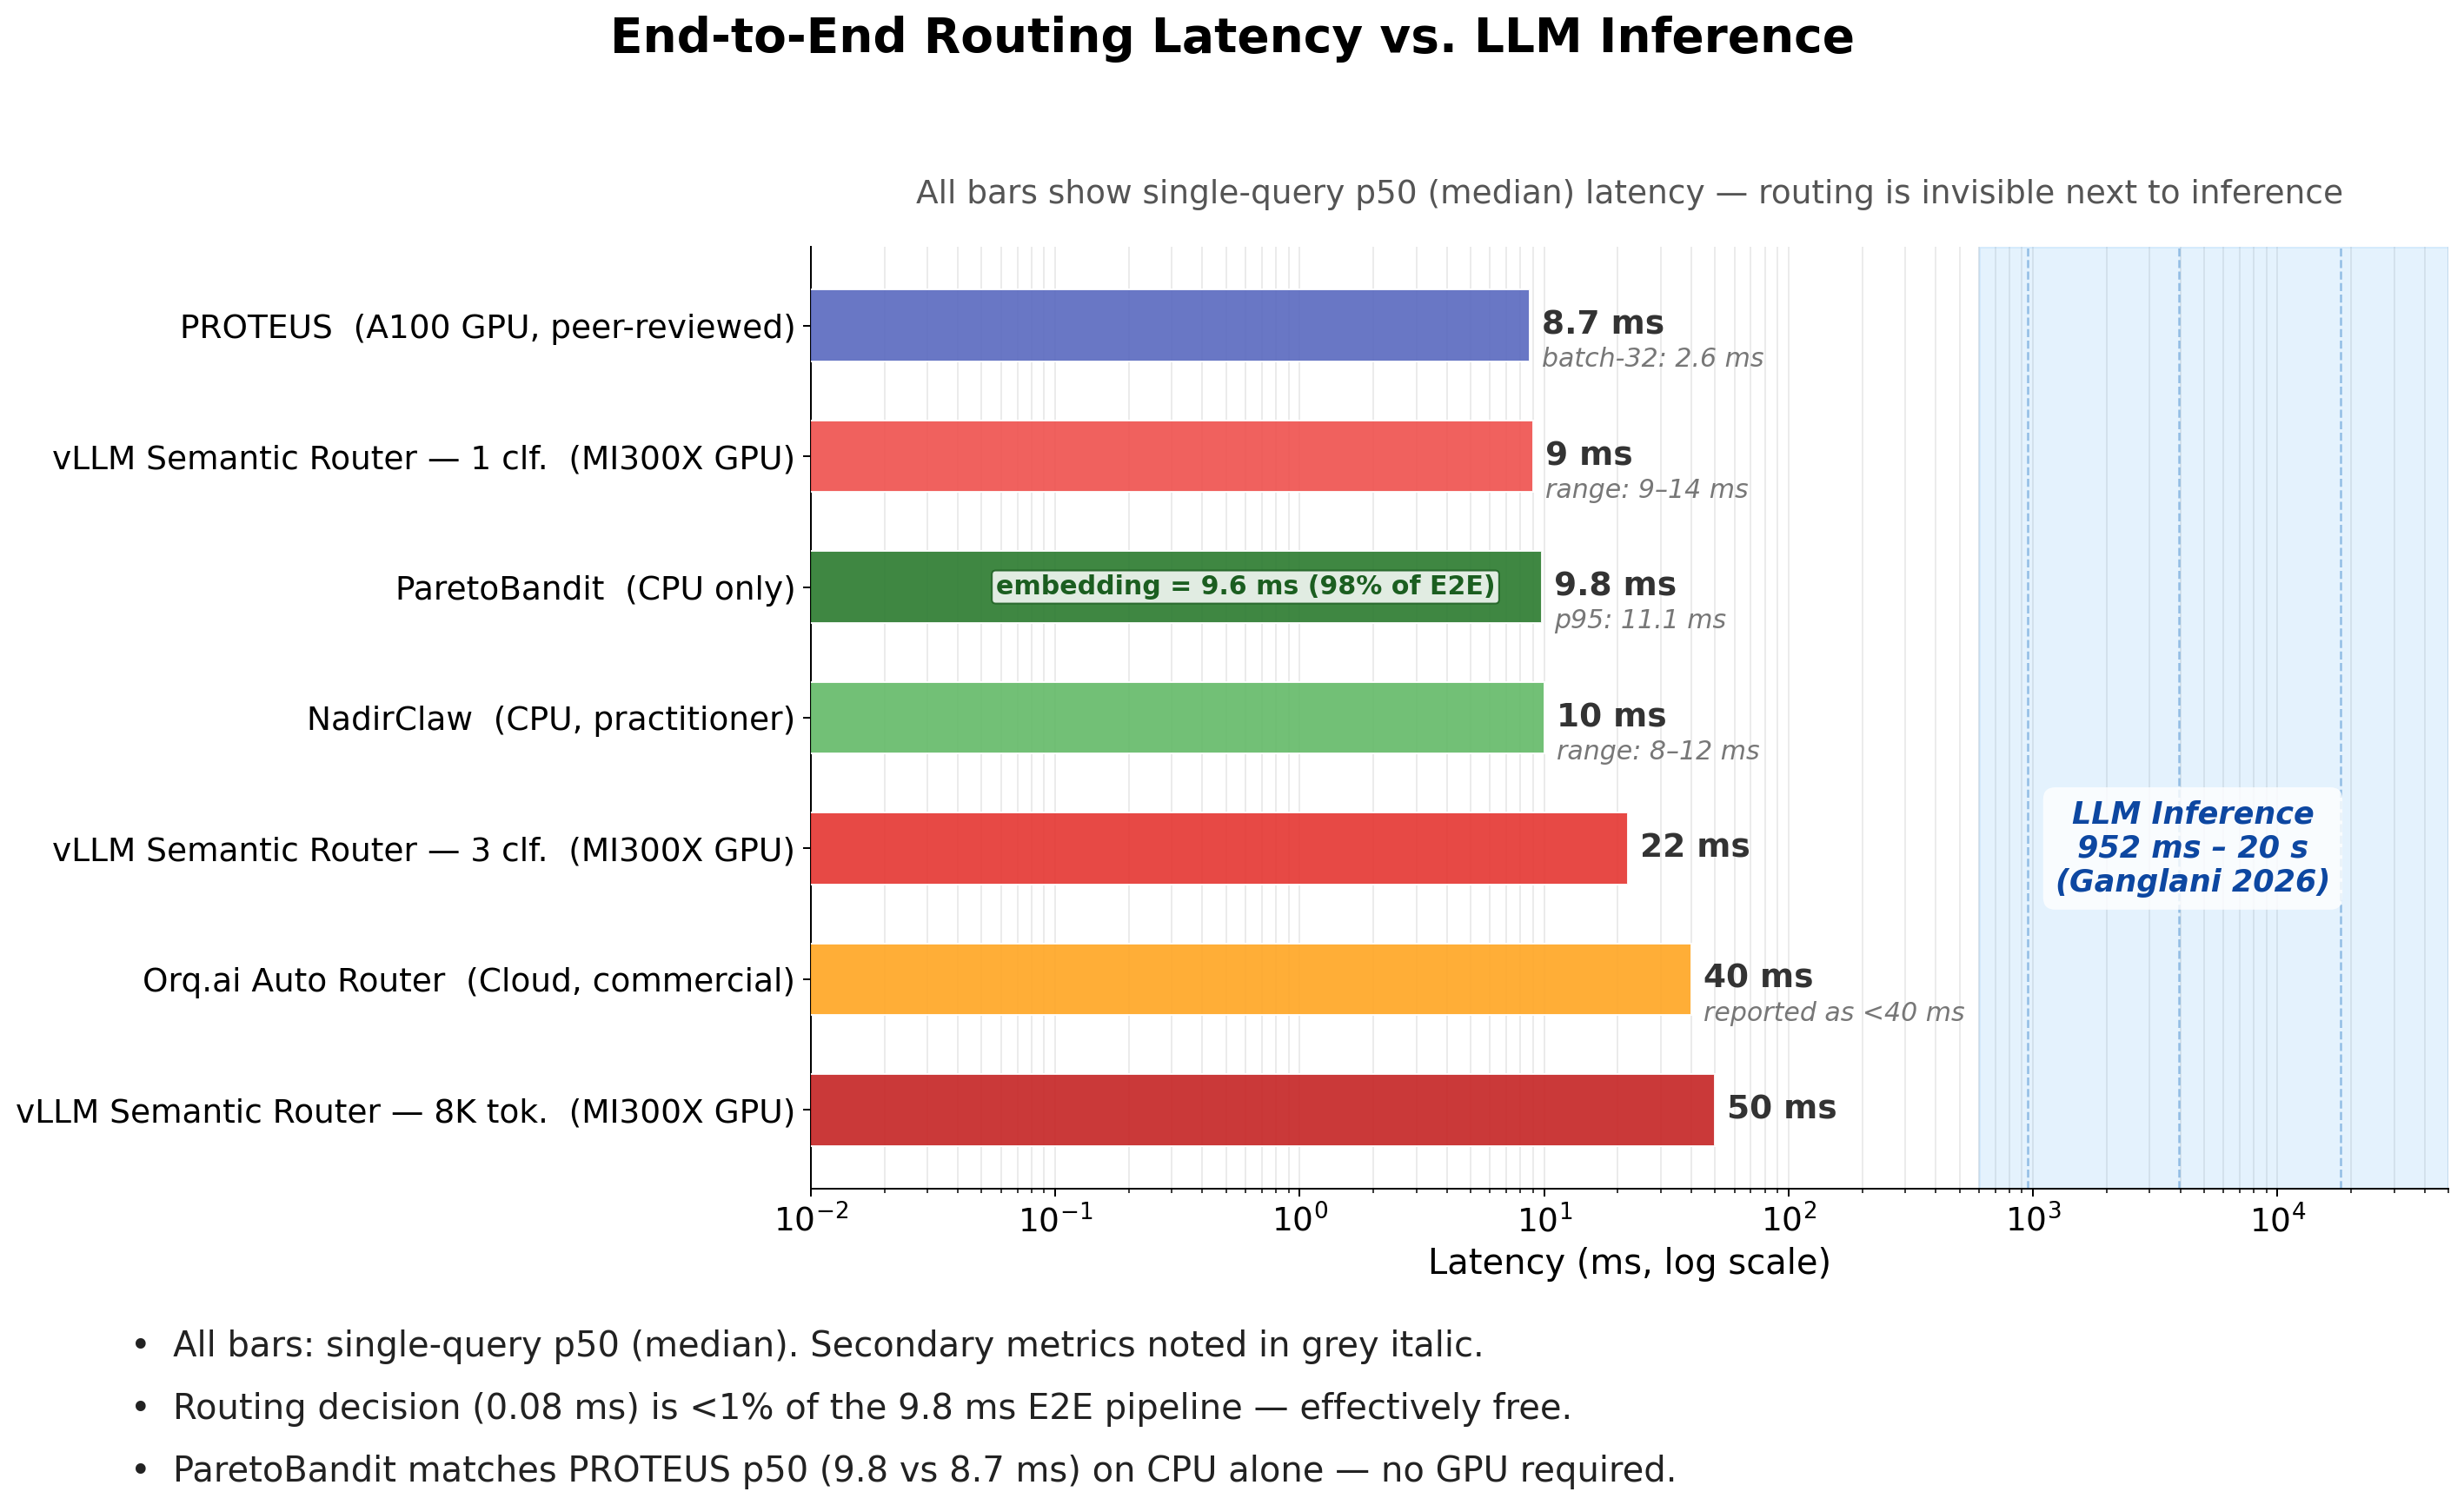
\includegraphics[width=\columnwidth]{../experiments/appendix/latency_benchmark/results/latency_spectrum_e2e.png}
\caption{End-to-end routing latency (p50, single query) for published
routing systems vs.\ LLM inference time.
ParetoBandit achieves $\latEteTotalMedianMs$\,ms on CPU only, matching
PROTEUS ($8.7$\,ms on an A100 GPU) without requiring GPU infrastructure
at the routing layer.
All routing latencies are orders of magnitude below LLM inference
(shaded region), confirming that the router is invisible to the end user.}
\label{fig:latency_spectrum_e2e}
\end{figure}

\paragraph{Routing overhead relative to LLM inference.}
Table~\ref{tab:overhead_vs_inference} contextualises ParetoBandit's
$\latEteTotalMedianMs$\,ms E2E overhead against production LLM API
latencies~\cite{ganglani2026llmlatency}.

\begin{table}[h]
\centering
\caption{ParetoBandit's routing overhead as a fraction of LLM inference
latency across representative models and prompt
lengths~\cite{ganglani2026llmlatency}.
\emph{TTFT} = time to first token (streaming); \emph{Total} = full response
latency.
Routing overhead is the $\latEteTotalMedianMs$\,ms end-to-end critical path (embedding +
PCA + \texttt{route()}) on CPU.}
\label{tab:overhead_vs_inference}
\small
\resizebox{\columnwidth}{!}{%
\begin{tabular}{@{}l l r r r@{}}
\toprule
\textbf{LLM} & \textbf{Prompt} & \textbf{TTFT (ms)} & \textbf{Total (ms)}
  & \textbf{Routing / Total} \\
\midrule
Claude Haiku 4.5 & short  & 639   & 952    & $1.40\%$ \\
Claude Haiku 4.5 & medium & 597   & 3{,}954  & $0.34\%$ \\
Gemini 2.5 Flash & medium & 730   & 1{,}729  & $0.77\%$ \\
GPT-4.1          & short  & 889   & 1{,}770  & $0.75\%$ \\
Claude Sonnet 4  & long   & 1{,}216 & 20{,}445 & $0.07\%$ \\
GPT-4.1 Mini     & long   & 2{,}501 & 18{,}075 & $0.07\%$ \\
\bottomrule
\end{tabular}
}
\end{table}

\noindent
Even against the fastest model and shortest prompt (Claude Haiku 4.5,
952\,ms), the full routing pipeline adds ${\sim}1.4\%$ overhead; for typical
workloads it contributes 0.3--0.8\%.  \textbf{The routing decision is
invisible to the end user.}
